\documentclass[12pt,letterpaper]{exam}
\usepackage[lmargin=1in,rmargin=1in,tmargin=1in,bmargin=1in]{geometry}
\usepackage{../style/exams}

% -------------------
% Course & Exam Information
% -------------------
\newcommand{\course}{MAT 100: Exam 1}
\newcommand{\term}{Fall -- 2022}
\newcommand{\examdate}{10/07/2022}
\newcommand{\timelimit}{85 Minutes}

\setbool{hideans}{true} % Student: True; Instructor: False

% -------------------
% Content
% -------------------
\begin{document}

\examtitle
\instructions{Write your name on the appropriate line on the exam cover sheet. This exam contains \numpages\ pages (including this cover page) and \numquestions\ questions. Check that you have every page of the exam. Answer the questions in the spaces provided on the question sheets. Be sure to answer every part of each question and show all your work.} 
\scores
%\bottomline
\newpage

% ---------
% Questions
% ---------
\begin{questions}

% Question 1
\newpage
\question[10] Showing all your work and finding an exact answer, compute the following:
	\begin{enumerate}[(a)]
	\item $3 (2^4) - 12$
	\item $\dfrac{(-2)^3 - 5 + 3 \cdot 6}{-5}$
	\item $\dfrac{5 \cdot 4 - 4 \cdot 3}{5 - 1}$
	\end{enumerate}



% Question 2
\newpage
\question[10] Define the following sets:
	\[
	\begin{aligned}
	A&= \{ -3,\; 1, \; 2,\; 3,\; 5,\; 10,\; 20,\; 30,\; 40,\; 50 \} \\
	B&= \{ -3,\; 3,\; 10,\; 50 \} \\
	C&= \{ 2,\; 5,\; 20,\; 40,\; 50 \} \\
	D&= \{ -3,\; 1,\; 5 \} \\
	E&= \{ 1,\; 2,\; 3,\; 5 \}
	\end{aligned}
	\]
Consider all these sets as subsets of $A$. Compute the following:
	\begin{enumerate}[(a)]
	\item $D^c$
	\item $C \cup D$
	\item $B \setminus C$
	\item $D \cap E$
	\item $|E|$
	\end{enumerate}



% Question 3
\newpage
\question[10] Determine whether the relation below is a function of not. Be sure to fully justify your response. If the relation is a function, find its domain, codomain, and range. 
	\[
	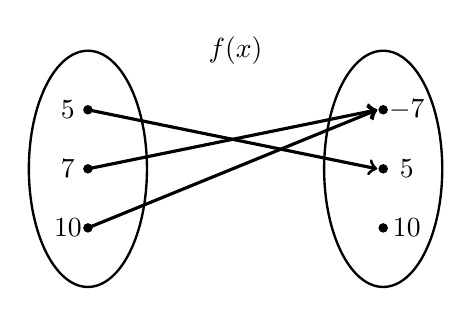
\begin{tikzpicture}[scale=0.75]
	\node at (2.5,2) {$f(x)$};
	% Ellipses
	\draw[line width=0.03cm] (0,0) circle (1 and 2);
	\draw[line width=0.03cm] (5,0) circle (1 and 2);
	
	% Nodes
	\draw[fill=black] (0,1) circle (0.07);
	\draw[fill=black] (0,0) circle (0.07);
	\draw[fill=black] (0,-1) circle (0.07);
	
	\draw[fill=black] (5,1) circle (0.07);
	\draw[fill=black] (5,0) circle (0.07);
	\draw[fill=black] (5,-1) circle (0.07);
	
	% Arrow
	\draw[line width=0.04cm,->] (0,1) -- (4.9,0);
	\draw[line width=0.04cm,->] (0,0) -- (4.9,1);
	\draw[line width=0.04cm,->] (0,-1) -- (4.9,1);
	
	% Labels
	\node at (-0.3,1) {$5\,$};
	\node at (-0.3,0) {$7\,$};
	\node at (-0.3,-1) {$10\,$};
	
	\node at (5.4,1) {$-7$};
	\node at (5.4,0) {$5$};
	\node at (5.4,-1) {$10$};
	\end{tikzpicture}
	\]



% Question 4
\newpage
\question[10] Explain why $f(x, y)= x^2 - y + 1$ is a function. Then showing all your work, find $f(0, 0)$, $f(0, -4)$, $f(3, 6)$, and $f(-2, 10)$. 



% Question 5
\newpage
\question[10] Showing all your work, find the following:
	\begin{enumerate}[(a)]
	\item 56\% of 920
	\item 150\% of 60
	\item 1\% of 840
	\end{enumerate}



% Question 6
\newpage
\question[10] Showing all your work, compute the following:
	\begin{enumerate}[(a)]
	\item 150 increased by 42\%
	\item 245 decreased by 20\%
	\item 660 increased by 125\%
	\end{enumerate}



% Question 7
\newpage
\question[10] Find the average value of the following numbers: $-7, -4.2, -1, 0, 2, 6, 10, 12$.



% Question 8
\newpage
\question[10] Suppose a student's course grade consists of the following weights: \par
	\begin{table}[!ht]
	\centering
	\begin{tabular}{rrcrr}
	Homework & 40\% & & Exam 2 & 15\% \\
	Quizzes & 5\% & & Final Exam & 17\% \\
	Exam 1 & 8\% & & Project & 15\% \\
	\end{tabular}
	\end{table} \par
Suppose also that a student had a 85.6\% homework average, 80\% quiz average, 92\% on exam 1, 87\% on exam 2, 79\% on the final, and 95\% on the project. Compute the student's course average to the nearest tenth of a percent. 



% Question 9
\newpage
\question[10] Suppose you take the courses shown below and receive the given letter grades. Showing all your work, compute your GPA to the nearest thousandth. The university's letter grade system is shown on the right below. \par
	\begin{table}[!ht]
	\centering
	\begin{tabular}{lrr}
	Course & Credits & Letter Grade \\ \hline
	Eastern Europe & 3 & B$-$ \\
	Modern American Literature & 3 & C$+$ \\
	Calculus~II & 4 & A\phantom{$-$} \\
	Chemistry~I & 4 & A$-$ \\
	Introduction to College Life & 1 & A\phantom{$-$} \\
	Freshman Seminar & 3 & B\phantom{$-$}
	\end{tabular} \hspace{1cm}
        \begin{tabular}{|l||c|l||c|} \hline
        A & 4.0 & C+ & 2.3 \\ \hline
        A-- & 3.7 & C & 2.0 \\ \hline
        B+ & 3.3 & C-- & 1.7 \\ \hline
        B & 3.0 & D & 1.0 \\ \hline
        B-- & 2.7 & F & 0.0 \\ \hline
        \end{tabular}
	\end{table}



% Question 10
\newpage
\question[10] Showing all your work, convert 648~in$^2$ to square feet. Recall that there are twelve inches in every foot.



% Question 11
\newpage
\question[10] Showing all your work, convert 9.5~km/hr to feet per minute. Note that 1~m is 3.28084~ft.



% Question 12
\newpage
\question[10] Suppose you are covering a wall with black and white checker tiles. The wall measures 40~ft across and is 9~ft tall. If each tile is 6~in by 6~in, how many tiles will you need to cover the wall? Suppose also that you can put tiles on the wall at a rate of 3~tiles per minute. How long will it take you to tile the wall? For both questions, be sure to show all your work and fully justify your answer. 



% Question 13
\newpage
\question[10] Showing all your work, find the volume of a cylinder that is measures 4~in across the bottom and is 11~in tall. 



% Question 14
\newpage
\question A city is laid out in a grid structure with street corners meeting at right angles, as shown below with the street labeled. Suppose you are standing at point $P$ and your friend is standing at point $Q$.
	\[
	\fbox{%
	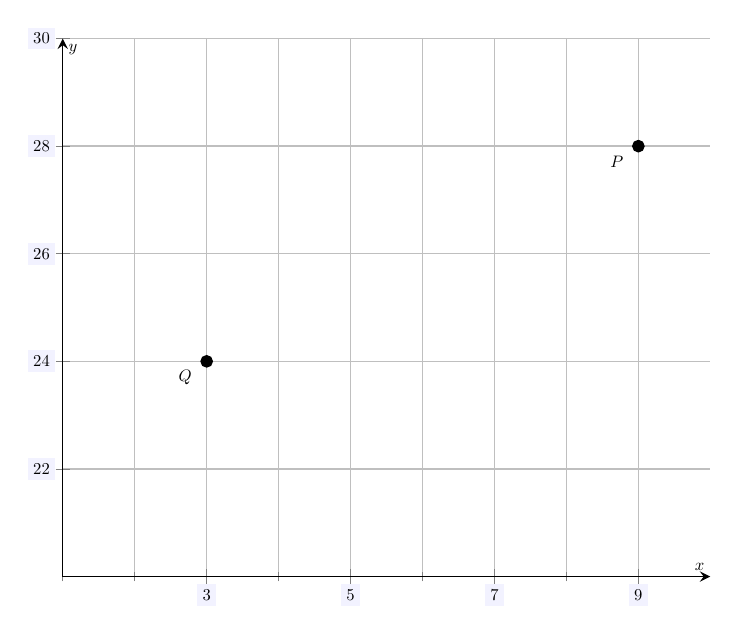
\begin{tikzpicture}[scale=1.2,every node/.style={scale=0.5}]
	\begin{axis}[
	grid=both,
	axis lines=middle,
	ticklabel style={fill=blue!5!white},
	xmin= 1, xmax=10,
	ymin= 20, ymax=30,
	xtick={1,3,5,7,9},
	ytick={20,22,24,26,28,30},
	minor tick = {-8,-7,...,8},
	xlabel=\(x\),ylabel=\(y\),
	]
	\node at (2.7,23.7) {$Q$};
	\draw[fill=black] (3,24) circle (0.06cm);
	\node at (8.7,27.7) {$P$};
	\draw[fill=black] (9,28) circle (0.06cm);
	\end{axis}
	\end{tikzpicture}
	}
	\]
\begin{parts}
\part[4] How many blocks are you from your friend `as the crow flies'?
\part[4] How many blocks are you from your friend using the taxicab metric?
\part[2] Supposing you can walk a block in 4~min and given your answer in (b), how long do you estimate that it will take you to walk to your friend?
\end{parts}



% Question 15
\newpage
\question[10] Showing all your work and fully explaining your approximation, estimate how many pet dogs there are in the United States. 


\end{questions}
\end{document}